%\documentclass[reponses, utf8, 11pt]{feuille}
\documentclass[utf8, 11pt]{feuille}

\newcommand{\titredutd}{\textbf{TD3 --- L'ensemble micro-canonique~: micro-états \& entropie}}

\begin{document}


\begin{tcolorbox}[
        colback=gray!20,
        colframe=gray!20,
        width=\dimexpr\textwidth\relax, 
        arc=0pt,outer arc=0pt,
        ]

\texttt{Seules les calculatrices non communicantes et les notes manuscrites personnelles sont autorisées.}

\texttt{Les exercices sont totalement indépendants.}

\texttt{On notera $k_B$ la constante de Boltzmann et $h$ la constante de Planck.}

\end{tcolorbox}



% ______________________________________________________________________________
\section{\soft~Fluctuation de moments magnétiques}

On considère un système de sept atomes. Le moment magnétique $\mu_i$ de chaque atome $i=1,2,\dots, 7$ fluctue et peut valoir $+\mu$ ou $-\mu$. Les interactions entre les moments magnétiques sont négligées, on suppose le champ magnétique extérieur nul. Le système est composé de deux sous-systèmes: le sous-système~I qui contient quatre atomes et le sous-système~II qui en contient trois. On suppose que tous les micro-états du système sont équiprobables

\question
Calculer le nombre $\varOmega$ de micro-états accessibles du système.
  
\question
Calculer la probabilité $Pr(M_I=-2\mu)$ pour que $M_I=-2\mu$, où $\displaystyle M_I=\sum_{i=1}^4 \mu_i$ est le moment total du sous-système~I. 

\question
Calculer la valeur moyenne $\langle M_I \rangle$ de $M_I$. 

\medskip

On suppose maintenant que l'on impose un moment magnétique total
$M_I+M_{II}$ égal à $\mu$. Tous les micro-états qui vérifient cette
contrainte sont équiprobables.

\question
Calculer le nouveau nombre $\varOmega$ de micro-états accessibles du système. 

\question
Calculer la nouvelle probabilité $Pr(M_I=-2\mu)$  pour que $M_I$=-2$\mu$. Quelle est la probabilité $Pr(M_{II}=3\mu)$ que $M_{II}=3\mu$ ? 

\question
Calculer la nouvelle valeur moyenne $\langle M_I \rangle$ de $M_I$. 

\elements{
\\
1 : 
$\varOmega=2^7=128$ ;
\\
2 : $M_I=-2\mu$, soit 4 micro-états tels que le sous-système I a 3 moments $-\mu$ et un moment $+\mu$ (par exemple $\downarrow \downarrow \uparrow \downarrow$), pour chacun de ces 4 micro-états, le sous-système II peut être dans $2^3$ micro-états, donc $Pr(M_I=-2\mu)=\frac{4\times 8}{128}=\frac{1}{4}$ (car les micro-états du système I$+$II sont équiprobables avec $p=1/128$).
\\
3 : Il y a 1 micro-état tel que $M_I=-4\mu$ ($\downarrow \downarrow \downarrow \downarrow$), 4 micro-états tels que $M_I=-2\mu$ ($\uparrow \downarrow \downarrow \downarrow$), ${4 \choose 2}=6$ micro-états tels que $M_I=0$ ($\uparrow \uparrow \downarrow \downarrow$), 4 micro-états tels que $M_I=+2\mu$ ($\uparrow \uparrow \uparrow \downarrow$) et 1 micro-état tel que $M_I=+4\mu$ ($\uparrow \uparrow \uparrow \uparrow$), pour chacun de ces micro-états de I, le sous-système II peut être dans $2^3$ micro-états, donc $\langle M_I \rangle=\frac{8}{128}(-4\mu\times 1 -2\mu \times 4 +0\times 6 + 2 \mu \times 4 +4 \mu \times 1)=0$ (résultat attendu par symétrie).
\\
4 : $M_I+M_{II}=\mu$, il y a donc 4 moments $+\mu$ et 3 moments $-\mu$ dans le système I$+$II, soit $\varOmega= {7 \choose 4}=35$.
\\
5 : $M_I=-2\mu$, soit 4 micro-états tels que le sous-système I a 3 moments $-\mu$ et un moment $+\mu$, un seul micro-état est alors accessible au sous-système II tel que $M_{II}=\mu-M_I=3\mu$ ($\uparrow \uparrow \uparrow$), donc $Pr(M_I=-2\mu)=\frac{4\times 1}{35}$ et $Pr(M_{II}=3\mu)=\frac{1\times 4}{35}$.
\\
6 : Les micro-états  accessibles du système I sont les mêmes qu'à la question 4, sauf le micro-état $\downarrow \downarrow \downarrow \downarrow$, car il n'y a que 3 moments $-\mu$ dans le système I$+$II. On a donc $Pr(M_I=-2\mu)=\frac{4\times 1}{35}$, $Pr(M_I=0)=\frac{6\times 3}{35}$, car ${4 \choose 2}=6$ micro-états tels que $M_I=0$ et 3 micro-états tels que $M_{II}=\mu$, $Pr(M_I=2\mu)=\frac{4\times 3}{35}$, car 4 micro-états tels que $M_I=2\mu$ et 3 micro-états tels que $M_{II}=-\mu$, $Pr(M_I=4\mu)=\frac{1\times 1}{35}$, car 1 micro-état tel que $M_I=4\mu$ et 1 micro-état tel que $M_{II}=-3\mu$ (on a bien la normalisation $Pr(M_I=-2\mu)+Pr(M_I=0)+Pr(M_I=2\mu)+Pr(M_I=4\mu)=1$). Ainsi  $\langle M_I \rangle=\frac{1}{35}( -2\mu \times 4 +0\times 18 + 2 \mu \times 12 +4 \mu \times 1)=\frac{20}{35}$.
}



% ______________________________________________________________________________
\section{\soft~Le cristal paramagnétique parfait}

Soit un système de $N$ spins $\frac12$ portés par des atomes localisés
aux n\oe uds d'un réseau cristallin et plongés dans un champ
magnétique $\mathbf{B}$. On néglige les interactions entre les
spins. Ce système de particules {\it indépendantes} est isolé à l'énergie
$E$, donnée par
$$
E = - \sum_{j=1}^{N} \mu B s_j \quad \textrm{avec} \quad s_j = \pm
1 \enspace .
$$

\question
Les atomes sont-ils discernables ou indiscernables ? 

\question
Quels sont les paramètres extérieurs ? 

\question
Pour commencer considérons $N=5$ spins isolés à l'énergie
  $E=-\mu B$. Quel est le nombre $\varOmega$ de micro-états accessibles
  au système ? Que vaut la moyenne $\langle s_j \rangle$ d'un spin ? 

\medskip

Généralisons au cas d'un système de $N$ spins indépendants à l'énergie $E$.

\question
Soit $N_+$ le nombre de spins parallèles au champ magnétique ($s_j=+1$) et $N_-$ le nombre de spins antiparallèles au champ magnétique ($s_j=-1$). Exprimer  $E$ en fonction de $N$ et $N_+$.  

\question
Quel est le nombre de micro-états accessibles $\varOmega (N,E)$ ?

\elements{
\\
1 : Les atomes étant localisés aux n\oe uds d'un réseau cristallin, ils sont discernables.
\\
2 : $B$.
\\
3 : Les micro-états accessibles ont trois spins $+1$ et deux spins $-1$ (par exemple $\uparrow \downarrow \uparrow \uparrow \downarrow$), $\varOmega$ est le nombre de façons de choisir trois spins parmi cinq (une fois choisis, on leur affecte la valeur $+1$, les deux spins restants valent nécessairement $-1$), soit $ \varOmega = {5 \choose 3} = \frac{5!}{3!\ 2!}=10$ (pour s'en convaincre, on peut facilement recenser les dix micro-états accessibles), $ \langle s_j \rangle = (+1)\frac{6}{10} + (-1) \frac{4}{10} =\frac{1}{5}$, car les 10 micro-états ont la même probabilité $p_m=1/10$ et un spin $j$ vaut $s_j=+1$ dans six micro-états et $s_j=-1$ dans quatre.
\\
4 : $N_-= N - N_+$, donc $ E = - \sum_{j=1}^{N} \mu B s_j = -\Big(+ \mu BN_+ -\mu B(N-N_+) \Big)=\mu B(N-2N_+)$.
\\
5 : $\varOmega (N,E)$ est égal au nombre de façons de choisir $N_+$ spins $+1$ parmi $N$, soit $ \varOmega (N,E)= {N \choose N_+}= \frac{N!}{N_+! (N-N_+)!}$, où $N_+=\frac{N}{2}\Big(1-\frac{E}{N\mu B}\Big)$.
}



% ______________________________________________________________________________
\section{\medium~Dés et billes}

\question
On lance trois dés (un rouge, un vert et un bleu) et on obtient un total de 11. Combien y a-t-il de façons différentes d'obtenir ce résultat ? 

\question
On répartit 11 billes entre trois boîtes (une rouge, une verte et une bleue), le nombre de billes par boîte n'étant pas limité. On caractérise une répartition par le nombre de billes présentes dans chaque boîte. On peut ne mettre aucune bille dans une boîte. Calculer le nombre de répartition différentes, selon que les billes sont discernables ou non. Comparer au cas précédent : qu'est-ce qui fait la différence ?

\question
On veut généraliser le calcul précédent au cas de $n$ billes et $N$ boîtes. En vous inspirant des trois dessins suivants, expliquer pourquoi ils représentent  tous le même système des $n$ billes dans $N$ boîtes, et en déduire que le nombre de répartition différentes cherché lorsque les billes sont indiscernables est donné par
$$
\frac{(N+n-1)!}{n! (N-1)!}
$$

\centerline{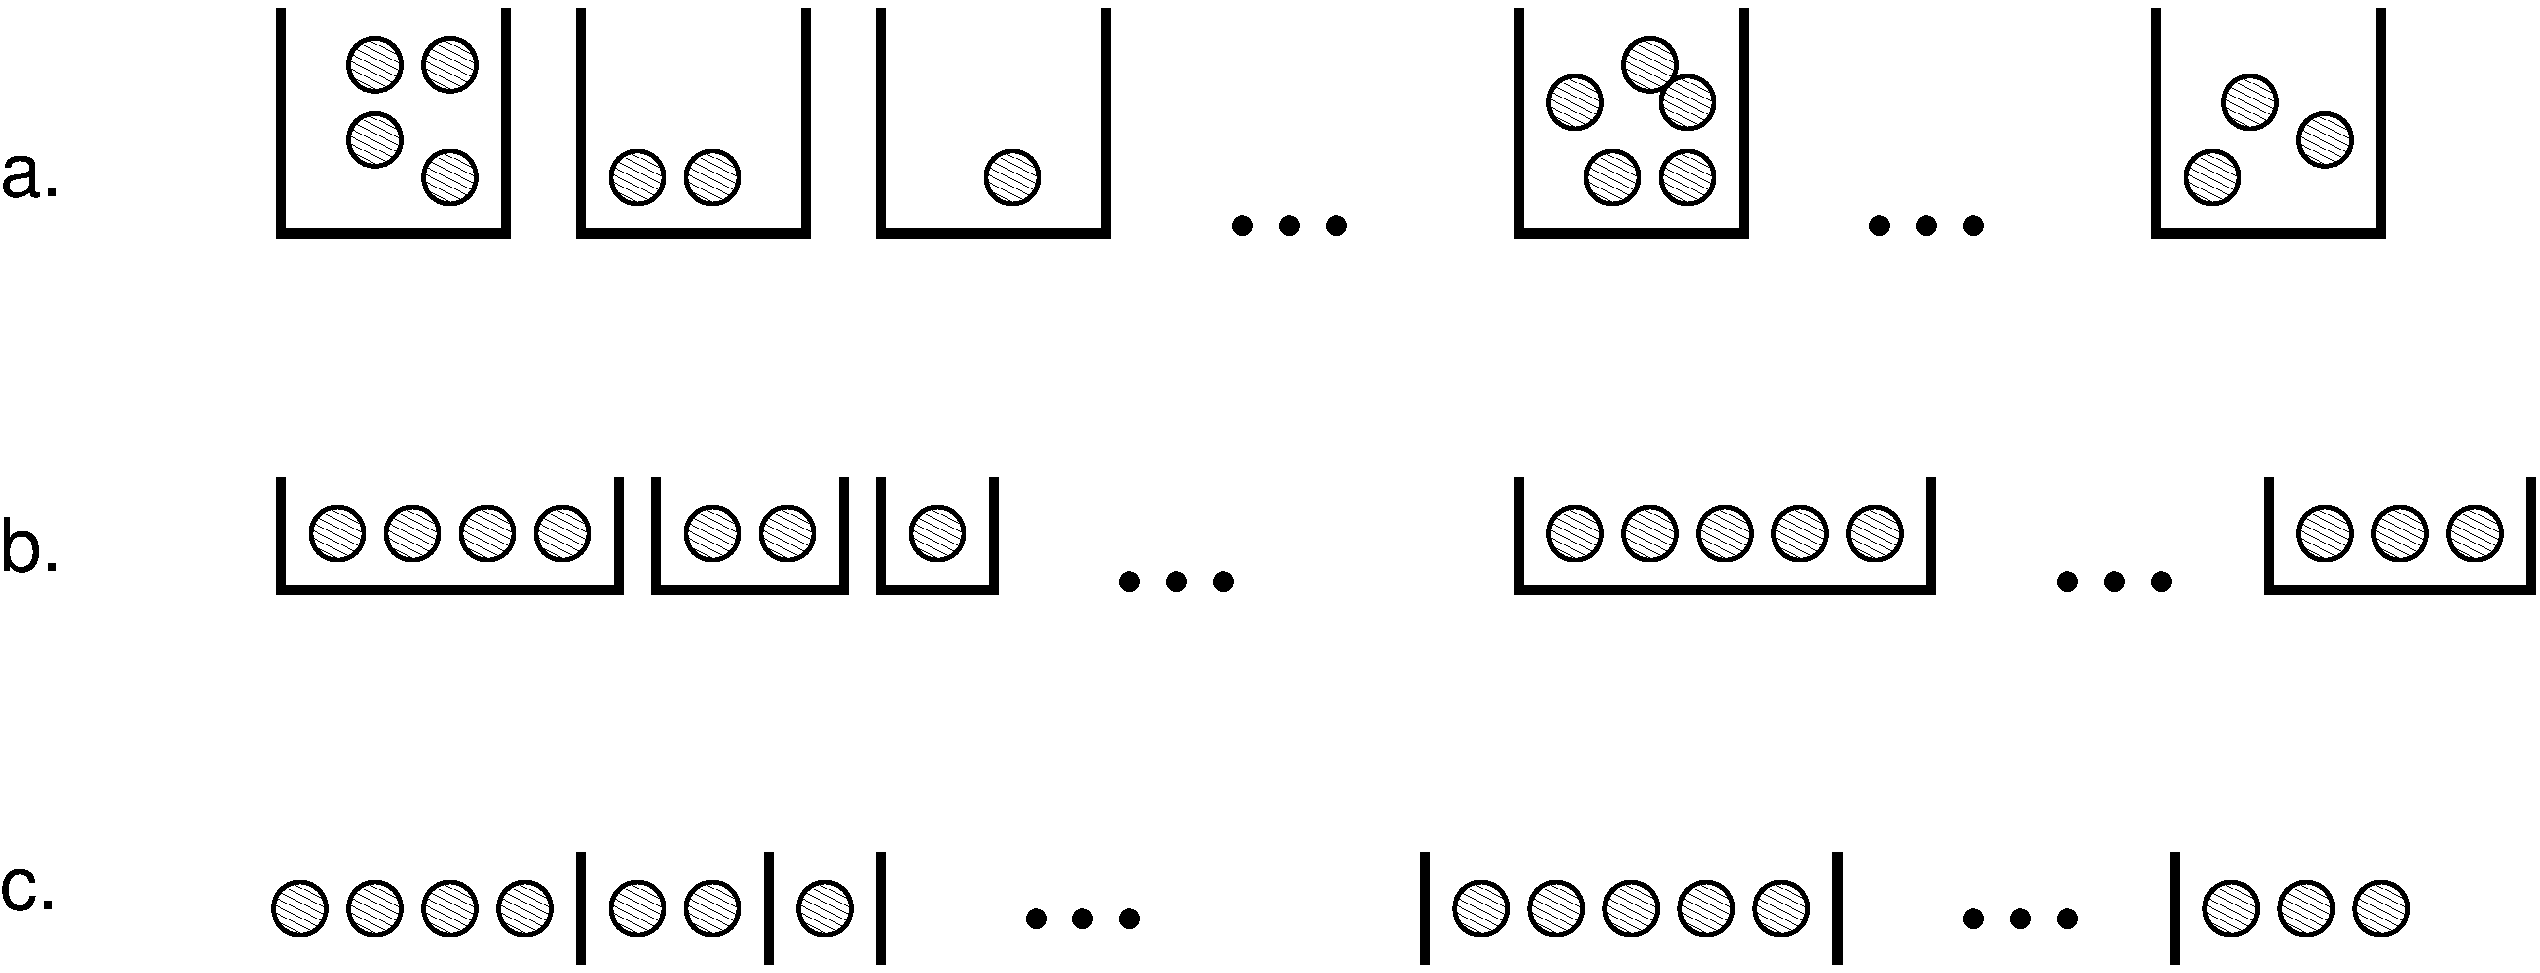
\includegraphics[height=.3\textwidth]{billes}}

\question
Comment est modifié ce résultat si les billes sont discernables ?

\question
Comment est modifié ce résultat si on ne peut pas mettre plus qu'une bille (indiscernable) par boîte ($N>n$) ?

\question
Qu'advient-il des résultats précédents lorsque $N\gg n$ ?



% ______________________________________________________________________________
\section{\medium~Ortho et para hydrogène}

Dans son état électronique fondamental, la molécule d'hydrogène $H_2$ peut exister sous deux formes : l'ortho-hydrogène où les spins des deux noyaux sont parallèles et le para-hydrogène, où ils sont antiparallèles. La forme para possède un seul état de spin dont on prendra l'énergie comme origine; la forme ortho présente trois états distincts, de même énergie $\epsilon >0$. On considère un échantillon d'hydrogène solide, constitué de $N$ molécules, fixes et discernables, faiblement couplées. On ne s'intéresse qu'aux états de spin ortho et para. Le système est isolé et son énergie (de spins) vaut $E (\gg \epsilon)$.

\question
Sur quel domaine peut-varier l'énergie $E$ ?

\question
Calculer le nombre $\Omega(E)$ de micro-états d'énergie $E = n \epsilon$.

\question
Dans l'hypothèse où $N$ et $n$ sont très grands, calculer l'entropie $S(E,N)$ du système.

\question
En déduire la température $T$ en fonction de $E, N, \epsilon$ et $k_B$.

\medskip

\`A l'équilibre thermodynamique, cette température de spins est égale à la température du matériau.

\question
\`A température ambiante, on mesure environ une répartition de 70\% d'ortho-H$_2$ et 30\% de para-H$_2$. En déduire un ordre de grandeur de l'écart énergétique $\epsilon$ entre les formes para et ortho.

\question
On lit souvent que \og l'ortho-hydrogène est instable à basse température, et se transforme spontanément en para-hydrogène avec le temps, ce qui libère de la chaleur indésirable. \fg \ Comprenez-vous cette assertion ? Estimer à 20 K la fraction ortho/para.







\end{document}
